\clearpage
\section{Расширенные эксперименты: влияние состава обучения}
\label{sec:additive_results}
Базовый эксперимент предыдущего раздела сравнивает четыре правила
на двух парах экспертов при 10 подвыборках без возвращения.
Далее исследуется полный набор восьми способов обучения:
на BANKING77 проверяются все 21 пары семи экспертов,
затем наблюдения проверяются на новой панели CLINC150.
Расширенный протокол использует 20 повторений и извлечения
с возвращением, позволяющие контролировать состав парной разметки.
Дополнительно анализируется качество конечных многоклассовых ответов.

\paragraph{Основные установленные эффекты.}
\begin{enumerate}
\item \textbf{Сравнительная деградация при harm-отборе.}
Изменение разности Direct--Weak-error равно \BankShiftEffect{} п.п.
для TF--IDF $\to$ frozen MiniLM на BANKING77 и \ClincShiftEffect{} п.п.
для TFfull $\to$ MiniLM на CLINC150 в рассматриваемых режимах.
\item \textbf{Выигрыш внутри gain-семейства.}
В harm8 raw на CLINC150 Hurdle превосходит Direct на
\HurdleSimpleEffect{} п.п.; изменение их сравнительной разности
между составами составляет \HurdleShiftEffect{} п.п.
\item \textbf{Прирост при корректировке известного отбора.}
Direct с IPW выигрывает у raw-обучения на \CorrectionEffect{} п.п.
в указанной CLINC150-паре.
\item \textbf{Преимущество в natural по конечным классовым ответам.}
Для CLINC150, TF3 $\to$ MiniLM, MSE-настройка,
Ternary превосходит Hurdle на \NaturalAccuracyEffect{} п.п. accuracy
и \NaturalFoneEffect{} п.п. macro-F1.
\end{enumerate}
Для каждого эффекта далее приведены условия, одновременные интервалы
и полная статистическая семья. Утверждения относятся к конкретным
конфигурациям, а не к универсальному рейтингу методов.

\section{Метод и теоретические основания}\label{sec:method}
\subsection{Оценивание полезности и решение при квоте}
Основная идея --- сначала оценить сравнительную полезность второго
ответа по доступным признакам, затем отделить обучение этой оценки
от выбора запросов при ограничении на число вызовов.
Исследуется выбор \emph{способа обучения} оценки: сравнительный
протокол меняет объём и состав разметки, проверяет взаимодействие
этих факторов с методом и оценивает выбор кандидата по отдельному dev.
Используются фиксированные эксперты и полностью парные метки;
статистическая независимость их ошибок не предполагается.
Признаки рассчитываются до второго вызова. Обучающий и эксплуатационный
потоки совпадают либо механизм изменения состава обучения известен.

Для пакета из $N$ запросов с условными полезностями $g_i=g(z_i)$
и ровно $k$ разрешёнными вызовами задача имеет вид
\begin{equation}\label{eq:topk}
\max_{r_i\in\{0,1\},\,\sum_i r_i=k}\ \sum_{i=1}^{N}r_i g_i.
\end{equation}
Предполагается, что остальные запросы пакета не дают дополнительной
информации об исходе объекта сверх $z_i$; это выполняется, например,
при независимых запросах. Решение --- выбрать $k$ наибольших $g_i$:
если выбран меньший элемент вместо большего, их обмен не уменьшает
цель. Это стандартное свойство квотного ранжирования, а не новый
теоретический результат. При ограничении \emph{не более} $k$ вызовов
отрицательную полезность эскалировать не следует; наши эксперименты
используют именно равную квоту, что важно для интерпретации вреда.

Если для всех объектов $|\widehat g_i-g_i|\le\varepsilon$,
разность ожидаемой accuracy оптимального и оценённого top-$k$ не больше
$2k\varepsilon/N$. Действительно, добавление и вычитание сумм
$\widehat g_i$ по двум наборам даёт два слагаемых, каждое ограничено
$k\varepsilon$; промежуточная разность неположительна по оптимальности
набора для $\widehat g$. Это условная граница: малая средняя MSE сама
по себе не гарантирует такую равномерную ошибку или верное ранжирование
около границы квоты.

\subsection{Модели и критерии обучения}
\textbf{Direct} --- линейная ridge-регрессия метки $D$ по
стандартизованным признакам. Квадратичная потеря на естественном потоке
минимизируется условным средним $g(z)$ в неограниченном классе функций;
линейный класс даёт регуляризованное приближение.
\textbf{Events} --- две logistic-регрессии событий $D=1$ и $D=-1$;
их разность используется как score. Каждая голова минимизирует
бинарную log-loss с L2-регуляризацией. Головы не обязаны давать
согласованную трёхклассовую вероятность; это ограничение параметризации.

\textbf{Weak-error} оценивает ошибку первой модели и вычитает среднюю
ошибку второй на fit. Вычитание константы не меняет ранжирование,
но score не равен условной полезности при неоднородной ошибке второго
эксперта. \textbf{Confidence} использует единицу минус максимальная
вероятность первого классификатора; не обучается и не рассматривается
как откалиброванный прогноз $D$.
Прямая оценка и разность двух \emph{ridge}-прогнозов с одинаковыми
данными и регуляризацией тождественны по линейности оператора решения.
Поэтому такое дублирование не образует содержательного нового метода.

Расширенная проверка включает весь исходный набор из восьми обучаемых
методов (таблица~\ref{tab:all_methods}), а не только direct/events.
Marginal обучает отдельные logistic-вероятности правильности экспертов.
Ternary использует softmax трёх значений $D$, joint --- четырёх
совместных исходов $(W,S)$. Hurdle отдельно оценивает вероятность
расхождения и направление среди расхождений. Soft-gain обучает
одну logistic-модель с мягкой меткой $(D+1)/2$ и возвращает
удвоенную вероятность минус единица. В неограниченном классе семь
gain-параметризаций нацелены на одну условную полезность;
конечные классы функций, потери, регуляризация и поддержка редких
событий могут давать различную чувствительность к обучению.

\begin{table}[htbp]\centering\small
\caption{Полный набор обучаемых методов. Число параметров при восьми
признаках указано формально, без общего стандартизатора, при наличии
всех классов; совпадение параметров не означает совпадения классов функций.}
\label{tab:all_methods}
\begin{tabular}{llr}
\toprule
Метод & Обучающие цели / прогноз & Параметров \\
\midrule
Weak-error & Ошибка первого минус средняя ошибка второго & 10 \\
Direct & Ridge-регрессия $D$ & 9 \\
Marginal & $P(S=1\mid z)-P(W=1\mid z)$, две logistic & 18 \\
Events & $P(D=1\mid z)-P(D=-1\mid z)$, две logistic & 18 \\
Ternary & Три класса $D$; разность крайних вероятностей & 27 \\
Joint & Четыре класса $(W,S)$; rescue минус harm & 36 \\
Hurdle & $P(D\ne0\mid z)[2P(D=1\mid D\ne0,z)-1]$ & 18 \\
Soft-gain & Мягкая метка $(D+1)/2$, прогноз $2\sigma-1$ & 9 \\
\bottomrule
\end{tabular}
\end{table}
Confidence и случайное ранжирование служат необучаемыми контролями.
Случайное правило не участвует в выборе кандидата или основной
семье статистических сравнений.

Пусть $u_i$ --- вес потери и $n$ --- число обучающих извлечений.
В direct минимизируется $n^{-1}\sum_i u_i(D_i-f_\theta(z_i))^2+
\lambda\|\theta_{\rm coef}\|^2$; в каждой logistic-голове ---
$n^{-1}\sum_i u_i\ell_i+\lambda\|\theta_{\rm coef}\|^2/2$.
Intercept не штрафуется. В коде это соответственно
$\alpha=n\lambda$ и $C=(n\lambda)^{-1}$.
Для ridge решается регуляризованная линейная система,
для logistic применяется L-BFGS; предупреждение о несходимости
останавливает новый эксперимент. Отсутствующее событие даёт нулевую
константу, единственный наблюдаемый класс --- соответствующую константу.
Общая сетка регуляризации настраивается по MSE на tuning-dev.

\subsection{Почему отбор исходов меняет обучающую цель}
Пусть $p_t(z)=P(D=t\mid z)$, $t\in\{-1,0,1\}$,
и обучающий поток $Q$ перевзвешивает исход множителем $a_t>0$.
Тогда по формуле Байеса
\begin{equation}\label{eq:selection_shift}
\begin{aligned}
q_t(z)&=\frac{a_t p_t(z)}{\sum_{u=-1}^{1}a_u p_u(z)},\\
g_Q(z)&=\frac{a_1p_1(z)-a_{-1}p_{-1}(z)}{\sum_{u=-1}^{1}a_u p_u(z)}.
\end{aligned}
\end{equation}
Невзвешенная регрессия теперь оценивает $g_Q$, а не $g_P$.
Усиление вредных исходов меняет и числитель, и нормировку,
поэтому может изменить знак и порядок полезности.
Даже одинаковое усиление двух ненейтральных исходов не обязательно
сохраняет ranking: при вероятностях $(p_1,p_{-1},p_0)=(0.2,0,0.8)$
и $(0.4,0.15,0.45)$ исходные полезности равны 0.20 и 0.25;
при множителях $(a_1,a_{-1},a_0)=(4,4,1)$ получаются
0.50 и приблизительно 0.377. Это иллюстрация известного механизма
смещения отбора \citep{nyberg2023exploring}, не заявление новой теоремы.

В контроле используется конечный размеченный пул размера $N_0$.
Каждая строка извлекается \emph{с возвращением} с известной
вероятностью $\rho_i=a_{D_i}/\sum_j a_{D_j}$.
Вес обратной вероятности извлечения (IPW) равен
$u_i=1/(N_0\rho_i)$. Для фиксированной функции потерь
\begin{equation}\label{eq:ipw}
\mathbb E_{I\sim\rho}[u_I\ell_I]
=\sum_{i=1}^{N_0}\rho_i\frac{\ell_i}{N_0\rho_i}
=\frac{1}{N_0}\sum_{i=1}^{N_0}\ell_i.
\end{equation}
Таким образом, восстанавливается риск исходного \emph{пула}.
Равенство не гарантирует несмещённости обученных коэффициентов,
оптимальности ранжирования или прироста accuracy на новом потоке.
Вес не нормируется по реализации; стандартизатор общий для
corrected/uncorrected и обучается на их одинаковых fit-строках.
Взвешивание может увеличивать вариативность потерь, а повторные извлечения
не создают новых уникальных примеров. Поэтому одновременно измеряются
число уникальных строк и $n_{\rm eff}=(\sum_i u_i)^2/\sum_i u_i^2$;
последнее характеризует неравномерность весов, а не число новых меток.
В расширенном контроле веса передаются во все восемь оценивателей.
Для условной головы hurdle дополнительно учитывается нормировка
условного потока: полный вес умножается на
$Q(D\ne0)/P_{\rm pool}(D\ne0)$, известные по пулу и отбору.
Это сохраняет масштаб условного риска и его регуляризации;
при отсутствии расхождений прогноз hurdle равен нулю.

\subsection{Алгоритм обучения и выбора}
\noindent\textbf{Вход:} размеченные непересекающиеся fit-пул,
tuning-dev, selector-dev; фиксированные эксперты и признаки;
квота, состав извлечений и сетка регуляризации.
\begin{enumerate}
\item Рассчитать парные исходы в fit-пуле и вероятности извлечений.
Получить fit-строки, сохранить их идентификаторы и веса.
\item Оценить стандартизацию только по fit. Для каждого метода
и значения регуляризации обучить кандидата, при коррекции передавая
веса в функцию потерь.
\item Выбрать регуляризацию по минимальной MSE на tuning-dev;
при точном равенстве предпочесть более сильную регуляризацию.
\item На selector-dev оценить доступных кандидатов при той же квоте.
В двухметодном контроле выбираются четыре natural-правила;
в полном --- восемь обучаемых и confidence для каждого варианта
состава отдельно. Выбрать максимальную accuracy; точные равенства
разрешать по заранее зафиксированному порядку, начиная с confidence.
Порядок указан в протоколе и не объявляется универсальным
ранжированием сложности методов.
\item Применить выбранный score к новому пакету и выбрать top-$k$
с общими независимыми ключами разрешения равенств. Не переобучать
роутер после выбора; test использовать только для оценки.
\end{enumerate}
\noindent\textbf{Выход:} стандартизатор, обученный score, параметр
регуляризации и выбранный метод. Для диагностического сравнения
сохраняются также все кандидаты.

Для $d$ признаков решение ridge имеет стоимость порядка
$O(nd^2+d^3)$, одна оценка функции/градиента logistic --- $O(nd)$;
полная стоимость зависит от числа итераций и проверок шага L-BFGS.
Сетка из четырёх значений умножает стоимость обучения на четыре.
Предсказание линейных голов стоит $O(Nd)$, сортировка пакета ---
$O(N\log N)$. Здесь $d=8$, поэтому повторное обучение роутеров
не требует повторного запуска дорогих экспертов.
Проверяемые следствия: сокращение train/test разрыва с ростом данных,
устранение смещения известной коррекцией и ненулевая ошибка выбора
метода на конечном selector-dev.

\section{Почему меняется квотное ранжирование}
\label{sec:ranking_shift}
Формула~\eqref{eq:selection_shift} позволяет уточнить механизм
сравнительной деградации на уровне идеальных условных целей.
Обозначим $h_i=P(D=-1\mid z_i)$ и $g_i=E[D\mid z_i]$.
Если только harm-исход получает множитель $a\ge1$, то
\begin{equation}\label{eq:harm_target}
g_{a,i}=\frac{g_i-(a-1)h_i}{1+(a-1)h_i}.
\end{equation}
Все знаменатели положительны. Приведение разности двух дробей
к общему знаменателю даёт точное тождество
\begin{equation}\label{eq:rank_numerator}
\begin{aligned}
\operatorname{sign}(g_{a,i}-g_{a,j})
&=\operatorname{sign}\bigl((g_i-g_j)+(a-1)B_{ij}\bigr),\\
B_{ij}&=h_j(1+g_i)-h_i(1+g_j).
\end{aligned}
\end{equation}
Квадратичные по $a$ произведения сокращаются. Поэтому при $g_i>g_j$
и $B_{ij}<0$ порядок меняется после единственного порога
$a_{ij}^{*}=1+(g_i-g_j)/(-B_{ij})$; при $B_{ij}\ge0$ он сохраняется.

\paragraph{Следствие для границы квоты.}
Пусть $\mathcal S$ --- исходный top-$k$ по $g$, причём все выбранные
объекты строго превосходят все невыбранные. Тогда
\begin{equation}\label{eq:critical_multiplier}
a_{\mathrm{crit}}=
\min_{\substack{i\in\mathcal S,\ j\notin\mathcal S\\B_{ij}<0}}
\left(1+\frac{g_i-g_j}{-B_{ij}}\right).
\end{equation}
Минимум по пустому множеству равен бесконечности.
До этого порога все сравнения через границу квоты сохраняют знак;
после него хотя бы один невыбранный объект превосходит выбранный.
В точке порога результат зависит от разрешения равенств.
Это доказывает условие изменения множества; величина потери accuracy
зависит также от исходного зазора полезностей.

\paragraph{Значение для выбора способа обучения.}
Порог определяется условными harm-вероятностями и зазорами
\emph{между объектами}, а не только средней ошибкой экспертов.
В приложении приведены две популяции с одной агрегированной таблицей
совместных исходов, но разной реакцией top-$k$ на harm-отбор.
Следовательно, диагностика выбора должна учитывать расположение
спасений и вреда относительно доступных признаков и границы квоты.
При этом семь идеальных gain-оценок имеют общую цель~\eqref{eq:harm_target};
различия между конечновыборочными реализациями проверяются экспериментально.
Условие выведено как алгебраическое следствие известного преобразования
при отборе, а не заявляется новым общим принципом или готовым
оценённым на данных правилом выбора. Помимо доказательства выполнены
20\,000 численных проверок попарного тождества и 250 проверок
первой смены top-$k$ на конечных популяциях.

\section{Экспериментальный протокол}
\label{sec:experiments_extended}
\subsection{Две задачи и фиксированные панели экспертов}
Используются BANKING77 \citep{review17} и CLINC150
\citep{larson2019clinc}. Первая задача содержит 77 банковских намерений,
вторая --- 150 намерений из десяти предметных областей; в CLINC
рассматривается только in-scope классификация. Второй датасет
введён после исследования BANKING77, по отдельному протоколу,
зафиксированному до обучения новой панели и просмотра её test-результатов.

В BANKING77 после удаления четырёх нормализованных повторов
9\,999 train-строк разбиты на expert-train 5\,999, calibration 1\,000,
router-fit 2\,000 и policy-dev 1\,000. Эксперты --- TF--IDF+LR,
BERT-tiny, frozen MiniLM+LR, tuned MiniLM и три TF--IDF+LR
с 1/3/10 размеченными примерами на класс. Используются все 21
фиксированная пара, включая три пары между low-label экспертами.
Обучение экспертов отделено от обучения роутеров.

В CLINC150 официальный train разделён на expert-pool 10\,500
и router-fit-pool 4\,500, очищенный dev содержит 2\,997 объектов.
Четыре новых эксперта --- TF--IDF+LR с 3 и 10 метками на класс,
TF--IDF+LR на полном expert-pool и frozen MiniLM с новой LR-головой.
Словарь low-label TF--IDF построен по текстам полного expert-pool;
меняется доступ к меткам, а не к неразмеченным текстам.
Из expert-pool 85\% служат внутреннему обучению, 15\% --- выбору $C$,
после чего выполняется refit; для low-label фиксировано $C=16$.
Используется прежний pretrained snapshot MiniLM, но supervised-головы
обучены на CLINC, без переноса BANKING77 голов. Проверены все шесть пар
в порядке TF3, TF10, TFfull, MiniLM. Этот порядок задаёт сравнение
панели; экономия фактической latency для low-label направлений
отдельно не измерялась.

Official test сохранены: 3\,080 запросов BANKING77 и 4\,500 CLINC150.
Дополнительные clean-test исключают обнаруженные нормализованные
пересечения и повторы: 3\,072 и 4\,497 объектов соответственно.
Для CLINC учитываются также точные текстовые совпадения с BANKING77.
Объекты обучающих частей различны; сохранение official test допускает
выявленные текстовые пересечения, поэтому clean-test служит отдельной
проверкой чувствительности. Ревизии источников и параметры подготовки
приведены в приложении.

\subsection{Общие кандидаты, составы и два критерия настройки}
Для всех восьми методов из таблицы~\ref{tab:all_methods} доступны
одни восемь признаков первой модели: максимальная, вторая и третья
вероятности, разность двух наибольших, нормированная энтропия,
сумма квадратов вероятностей и log1p длины текста в символах и словах.
Признаки и ответ второго эксперта при выборе недоступны.
Стандартизатор оценивается только по fit.

Fit формируется извлечениями с возвращением; одинаковые случайные
числа связывают сравниваемые условия. Natural означает равномерный
отбор из router-fit-pool. В harm8 вероятность строки с $D=-1$
увеличивается множителем 8 относительно остальных исходов;
\emph{raw} и \emph{IPW} используют одни извлечения и стандартизатор,
но разные веса потери. Отбор выполняется по заранее известным
парным исходам всего пула и не моделирует бесплатное приобретение меток.

BANKING77 проверяется по полной сетке: fit 200/500/1\,000,
20 seeds, квоты 10/20/40\%, семь составов natural/rescue2/rescue8/
harm2/harm8/discordant8/neutral8 и четыре сильных состава с IPW.
Получены 110\,880 выбранных роутеров после 443\,520 кандидатов
регуляризации. На CLINC150 используются fit 200/1\,000, 20 seeds,
те же квоты и natural/raw-harm8/IPW-harm8: 23\,040 обученных кандидатов.

Общая сетка $\lambda\in\{0.001,0.01,0.1,1\}$ настраивается на
естественном tuning-dev размера $n/2$. В BANKING77 используется MSE
прогноза прироста. В CLINC150 одни и те же обученные кандидаты
выбираются двумя способами: по MSE или по accuracy каскада
при заданной квоте. Второй критерий выбирает $\lambda$ отдельно
для каждой квоты; точные равенства разрешаются в пользу более сильной
регуляризации. Это меняет критерий выбора, а не вычислительный
бюджет обучения. Отдельные 500 dev-объектов используются selector
для выбора из восьми методов и confidence. Test не входит в выбор.

\subsection{Контрасты и учёт неопределённости}
Основной режим всех новых сравнений --- fit1000, 20\% вызовов,
official test, средние по 20 обучениям. При этом требуется ровно
616 вторых вызовов в BANKING77 и 900 в CLINC150.
Пусть $A_{s,m}$ --- средняя accuracy метода $m$ при составе $s$.
Различаются простой эффект в одном составе и взаимодействие:
\begin{equation}\label{eq:extended_interaction}
\begin{aligned}
\delta_{s;m,r}&=A_{s,m}-A_{s,r},\\
\Delta_{m,r}&=\delta_{\mathrm{harm8\ raw};m,r}
                 -\delta_{\mathrm{natural};m,r}.
\end{aligned}
\end{equation}
Положительное $\Delta$ означает улучшение \emph{относительного}
качества $m$ против $r$ при изменении состава. Оно может возникнуть,
когда оба метода ухудшаются, но один теряет меньше. Отдельно
проверяется эффект IPW минус raw одного метода на тех же данных.

\begin{table}[htbp]\centering\small
\caption{Статистические семьи. Все интервалы в статье учитывают полную
семью своего этапа; примеры не образуют новой уменьшенной поправки.}
\label{tab:families}
\begin{tabular}{llrp{.37\linewidth}}
\toprule
Код & Этап & Контрастов & Перевыборка и область \\
\midrule
B & BANKING77 & 5\,691 & 2\,000 paired crossed повторов;
простые эффекты, взаимодействия, профили, IPW, selector \\
C & CLINC150 & 1\,698 & 2\,000 повторов и одно уточнение до
10\,000; оба tuning-критерия, простые эффекты и взаимодействия \\
M & Multiclass & 3\,564 & 2\,000 class-stratified paired crossed
повторов; natural, три метрики, оба датасета \\
\bottomrule
\end{tabular}
\end{table}

В каждой семье используются общие перевыборки seeds и test-запросов
для сравниваемых методов, точный пересчёт top-$k$ с кратностями
и одна centered max-$|t|$ поправка. Одновременные интервалы имеют
номинальное покрытие 95\%. Эксперты, обученные scores и сделанный
выбор по dev условно фиксированы. Для C приведены интервалы
уточнённого расчёта, а исходные интервалы и все шесть изменений
граничного статуса сохранены; основные выделенные эффекты значимы
в обоих расчётах. Уточнение Monte-Carlo точности не является
повторным экспериментом на новых данных.

Семья M дополнительно сохраняет support каждого истинного класса
при перевыборке запросов. Она оценивает accuracy, macro-precision
и macro-F1 в natural; прочие условия многоклассового анализа
рассматриваются описательно. Разные семейства имеют разные составы
и процедуры перевыборки, поэтому их статусы значимости не используются
как тест различия датасетов или tuning-критериев.

\section{Установленные улучшения и ухудшения}
\label{sec:positive_evidence}
Таблица~\ref{tab:main_effects} объединяет конкретные эффекты,
на которых основаны содержательные выводы. Для каждого эффекта
сохранены исходный контраст, направление сравнения и полная семья.
Это выбранные иллюстрации общей проверки, а не восемь независимых
репликаций; полные подсчёты приведены в приложении.

\begin{table}[htbp]\centering\footnotesize
\caption{Основные подтверждённые эффекты при fit1000 и квоте 20\%.
Interaction означает изменение разности между natural и harm8 raw.
Пары: B --- TF--IDF $\to$ frozen MiniLM; C --- TFfull $\to$ MiniLM,
кроме Ternary--Direct (TF10 $\to$ TFfull); M --- TF3 $\to$ MiniLM.
В C используется accuracy-настройка, в B и M --- MSE.
Знак соответствует первому методу минус второй.}
\label{tab:main_effects}
\begin{tabular}{lcrr}
\toprule
Сравнение / эффект & Семья & П.п. & 95\% интервал \\
\midrule
BANKING77: Direct--Weak-error, interaction & B & -4{,}87 & [-7{,}34; -2{,}40] \\
CLINC150: Direct--Weak-error, interaction & C & -2{,}00 & [-3{,}34; -0{,}66] \\
CLINC150: Hurdle--Direct, harm8 & C & 0{,}85 & [0{,}03; 1{,}66] \\
CLINC150: Hurdle--Direct, interaction & C & 0{,}87 & [0{,}06; 1{,}68] \\
CLINC150: Ternary--Direct, interaction & C & 0{,}77 & [0{,}11; 1{,}43] \\
CLINC150: Direct, IPW--raw & C & 2{,}04 & [0{,}68; 3{,}40] \\
CLINC150: Ternary--Hurdle, accuracy & M & 0{,}29 & [0{,}02; 0{,}57] \\
CLINC150: Ternary--Hurdle, macro-F1 & M & 0{,}33 & [0{,}04; 0{,}63] \\
\bottomrule
\end{tabular}

\end{table}

\subsection{BANKING77: отбор вызывает сравнительную деградацию gain-методов}
В полном сравнении BANKING77 harm8 без коррекции ухудшает
семь gain-параметризаций относительно обучаемого Weak-error
на четырёх из 21 проверенной пары: TF--IDF $\to$ frozen MiniLM,
TF--IDF $\to$ tuned MiniLM, BERT-tiny $\to$ frozen MiniLM
и TF--IDF с 3 $\to$ 10 метками на класс.
Получены 28 взаимодействий против Weak-error; ещё 28 относятся
к тем же методам против неизменного confidence.
Последний является контролем, поскольку не зависит от router-fit.

В примере TF--IDF $\to$ frozen MiniLM accuracy Direct меняется
с 91,44\% на 86,56\%, а Weak-error --- с 91,26\% на 91,25\%.
Изменение Direct--Weak-error равно \BankShiftEffect{} п.п.,
одновременный интервал $\BankShiftCI$.
Таким образом, найден именно сдвиг сравнительного качества,
а не только описательная разница двух средних.
Аналогичные взаимодействия в этой паре установлены для остальных
шести gain-методов. В семье B также подтверждены 28 ухудшений
raw-обучения относительно natural через контрасты с фиксированным
confidence и 34 положительных эффекта коррекции IPW относительно raw.

\begin{table}[htbp]\centering\small
\caption{BANKING77, TF--IDF $\to$ frozen MiniLM: средняя accuracy
в трёх составах, 20 обучений. IPW проверяется на тех же
harm8-извлечениях. Числа в таблице описательные; статистические
утверждения опираются на семью B.}
\label{tab:bank_extended}
\begin{tabular}{lrrr}
\toprule
Метод & Natural, \% & Harm8 raw, \% & Harm8 IPW, \% \\
\midrule
Weak-error & 91{,}26 & 91{,}25 & 91{,}25 \\
Direct & 91{,}44 & 86{,}56 & 91{,}49 \\
Marginal & 91{,}36 & 86{,}50 & 91{,}51 \\
Events & 91{,}45 & 86{,}50 & 91{,}52 \\
Ternary & 91{,}46 & 86{,}61 & 91{,}53 \\
Joint & 91{,}43 & 86{,}61 & 91{,}50 \\
Hurdle & 91{,}34 & 86{,}61 & 91{,}50 \\
Soft-gain & 91{,}37 & 86{,}52 & 91{,}49 \\
Confidence & 90{,}68 & 90{,}68 & 90{,}68 \\
\bottomrule
\end{tabular}

\end{table}

\subsection{CLINC150: воспроизведение сравнительной деградации}
На CLINC150 TFfull $\to$ MiniLM при MSE-настройке Direct меняется
с 94,68\% на 92,78\%, Weak-error --- с 94,71\% на 94,74\%.
При настройке по квотной accuracy Direct меняется с 94,68\%
на 92,69\%, Weak-error --- с 94,70\% на 94,71\%.
Для второго варианта изменение Direct--Weak-error равно
\ClincShiftEffect{} п.п., интервал $\ClincShiftCI$,
скорректированное $p=\ClincShiftP$.
Следовательно, обнаруженный тип сравнительной деградации
воспроизводится в новой панели и сохраняется при эксплуатационном
критерии настройки. Это проверка конкретного явления на втором
датасете, а не усреднение независимых эффектов по всем парам.

\begin{table}[htbp]\centering\small
\caption{CLINC150, TFfull $\to$ MiniLM: средняя accuracy,
accuracy-настройка, fit1000, квота20\%, 20 обучений.}
\label{tab:clinc_extended}
\begin{tabular}{lrrr}
\toprule
Метод & Natural, \% & Harm8 raw, \% & Harm8 IPW, \% \\
\midrule
Weak-error & 94{,}70 & 94{,}71 & 94{,}71 \\
Direct & 94{,}68 & 92{,}69 & 94{,}74 \\
Marginal & 94{,}69 & 92{,}95 & 94{,}72 \\
Events & 94{,}68 & 92{,}88 & 94{,}71 \\
Ternary & 94{,}69 & 92{,}92 & 94{,}71 \\
Joint & 94{,}68 & 92{,}94 & 94{,}71 \\
Hurdle & 94{,}66 & 93{,}54 & 94{,}73 \\
Soft-gain & 94{,}65 & 92{,}72 & 94{,}71 \\
Confidence & 94{,}47 & 94{,}47 & 94{,}47 \\
\bottomrule
\end{tabular}

\end{table}

\subsection{Внутри gain-семейства: Hurdle теряет меньше, чем Direct}
\textbf{В harm8 raw Hurdle превосходит Direct на
\HurdleSimpleEffect{} п.п.} Для TFfull $\to$ MiniLM
его accuracy составляет 93,54\% против 92,69\% у Direct.
Простой одновременный интервал разности Hurdle--Direct равен
$\HurdleSimpleCI$, скорректированное $p=\HurdleSimpleP$.
На natural средние составляют 94,66\% и 94,68\% соответственно.
Отдельный тест взаимодействия даёт
$\Delta_{\mathrm{Hurdle,Direct}}=\HurdleShiftEffect$ п.п.,
интервал $\HurdleShiftCI$, $p=\HurdleShiftP$.
Тем самым установлены одновременно выигрыш Hurdle в данном
harm-режиме и изменение относительного качества между составами.
Поскольку оба метода теряют относительно natural, интерпретация
этого результата --- \emph{меньшая деградация Hurdle}.

Всего при accuracy-настройке подтверждены восемь из 126
gain-only взаимодействий на трёх парах: TF3 $\to$ TF10,
TF10 $\to$ TFfull и TFfull $\to$ MiniLM.
Все восемь сохраняются при увеличении числа bootstrap-повторов
с 2\,000 до 10\,000; полный список дан в приложении.
Например, для TF10 $\to$ TFfull изменение Ternary--Direct
равно \TernaryShiftEffect{} п.п. с интервалом $\TernaryShiftCI$.
Следовательно, неодинаковая чувствительность наблюдается
не только между gain-целью и прогнозом ошибки первого эксперта,
но и между реализованными параметризациями одной идеальной полезности.

\begin{figure}[htbp]\centering
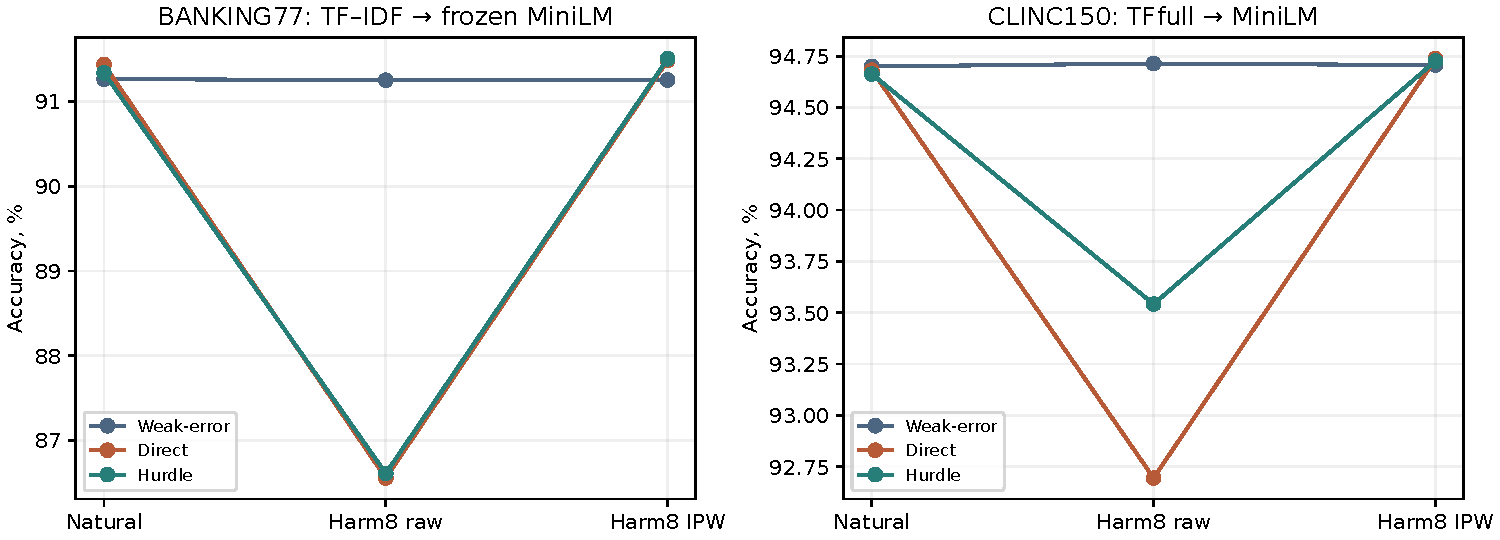
\includegraphics[width=\linewidth]{additions/figures/composition_effects.pdf}
\caption{Изменение средней accuracy при natural, harm8 raw и harm8 IPW.
Слева --- BANKING77, MSE-настройка; справа --- CLINC150,
accuracy-настройка. Линии показывают средние, без доверительных полос;
неопределённость соответствующих контрастов приведена в
таблице~\ref{tab:main_effects}.}
\label{fig:composition_extended}
\end{figure}

\subsection{Коррекция даёт измеримый прирост над raw-обучением}
В той же паре CLINC150 IPW повышает accuracy Direct с 92,69\%
до 94,74\%: эффект равен \CorrectionEffect{} п.п., интервал
$\CorrectionCI$, $p=\CorrectionP$.
Raw и IPW используют одинаковые fit-строки, признаки,
стандартизацию и сетку регуляризации; меняются веса обучающей потери,
а регуляризация выбирается по одному и тому же правилу.
Это контролируемое улучшение полного способа обучения с коррекцией.

Содержательный смысл состоит в восстановлении качества,
утраченного при известном смещении: natural-среднее Direct равно
94,68\%. Сравнение не следует представлять как выигрыш нового
роутера над естественным обучением. Возвращение средних к исходному
уровню и установленный IPW--raw эффект согласуются с изменением
условной цели в формуле~\eqref{eq:selection_shift}.
Поэтому при выборе по отобранной разметке нужны оба контроля:
простой обучаемый Weak-error и корректно взвешенные gain-кандидаты.

\section{Качество конечного многоклассового ответа}
\label{sec:multiclass_extended}
\subsection{Преимущество Ternary на естественном составе}
В отдельной общей семье M для CLINC150, TF3 $\to$ MiniLM,
natural, fit1000, квота20\%, MSE-настройка
\textbf{Ternary превосходит Hurdle одновременно по accuracy и macro-F1}.
Разница accuracy равна \NaturalAccuracyEffect{} п.п. с одновременным
интервалом $\NaturalAccuracyCI$ и $p=\NaturalAccuracyP$;
разница macro-F1 --- \NaturalFoneEffect{} п.п., интервал
$\NaturalFoneCI$, $p=\NaturalFoneP$.
Это пример прямого выигрыша одного gain-метода над другим
без искусственного изменения состава обучения.

\begin{table}[htbp]\centering\small
\caption{CLINC150, TF3 $\to$ MiniLM, natural, MSE-настройка:
многоклассовые метрики, средние по 20 обучениям.
Статистически установлен контраст Ternary--Hurdle;
таблица остальных кандидатов показывает полный контекст сравнения.}
\label{tab:natural_multiclass}
\begin{tabular}{lrrr}
\toprule
Метод & Accuracy, \% & Macro-P, \% & Macro-F1, \% \\
\midrule
Weak-error & 71{,}387 & 73{,}083 & 70{,}962 \\
Direct & 71{,}923 & 73{,}723 & 71{,}650 \\
Marginal & 71{,}373 & 73{,}073 & 70{,}947 \\
Events & 71{,}386 & 73{,}079 & 70{,}962 \\
Ternary & 71{,}603 & 73{,}321 & 71{,}212 \\
Joint & 71{,}577 & 73{,}275 & 71{,}176 \\
Hurdle & 71{,}310 & 73{,}011 & 70{,}878 \\
Soft-gain & 71{,}479 & 73{,}140 & 71{,}088 \\
Confidence & 71{,}911 & 73{,}812 & 71{,}788 \\
\bottomrule
\end{tabular}

\end{table}

\subsection{Какая информация добавляется к accuracy}
Метрики рассчитаны по истинным классам \emph{итогового ответа каскада}.
Восстановлены argmax-метки экспертов и решения маршрутизатора,
сохранены исходные tie-breaking и выбранные dev-параметры.
Всего пересчитаны 842\,760 строк скалярных метрик всех сохранённых
условий двух исследований. Для 42\,079 уникальных основных политик
классовые precision, recall и F1 независимо сверены со sklearn;
accuracy, спасения, вред и число вызовов воспроизвели прежние результаты.
На новых метриках роутеры не перенастраивались.

Для класса $c$ используются
\begin{equation}
P_c=\frac{TP_c}{TP_c+FP_c},\qquad
R_c=\frac{TP_c}{TP_c+FN_c},\qquad
F1_c=\frac{2TP_c}{2TP_c+FP_c+FN_c}.
\end{equation}
Нулевой знаменатель даёт 0; в усреднение входят все известные классы.
Macro-F1 --- среднее $F1_c$, а не гармоническое средних $P_c$ и $R_c$.
В single-label классификации без отказа micro-P/R/F1 и weighted-recall
совпадают с accuracy. Official test сбалансирован:
77 классов по 40 объектов в BANKING77 и 150 по 30 в CLINC150.
Поэтому здесь дополнительно macro-recall совпадает с accuracy,
а weighted-P/F1 --- с macro-P/F1. Новая агрегированная информация
содержится прежде всего в macro-precision и macro-F1.

Семья M включает все 36 попарных сравнений восьми обучаемых методов
и confidence в 33 конфигурациях: 21 BANKING77 и шесть CLINC150
при двух критериях настройки. Три метрики дают 3\,564 контраста;
bootstrap сохраняет support каждого класса. Найденное преимущество
Ternary относится к одному конкретному режиму и одной семье;
accuracy и macro-F1 оцениваются на тех же ответах и не являются
независимыми воспроизведениями.

\subsection{Разнонаправленные классовые эффекты при близких средних}
Другой описательный пример --- BANKING77, TF--IDF с одной меткой
на класс $\to$ tuned MiniLM. На natural Weak-error и Direct имеют
accuracy 42,742\% и 42,766\%, macro-precision 46,908\% и 47,446\%,
macro-F1 42,660\% и 42,827\%. Разница accuracy в 0,024 п.п.
соседствует с разницей macro-precision в 0,538 п.п.
Это возможно, потому что замена одной неправильной метки другой
меняет FP отдельных классов, сохраняя общую правильность.

Для класса \texttt{country\_support} F1 Weak-error и Direct
составляет 51,429\% и 39,530\%; для класса пополнения баланса
после чека или наличного депозита --- 40,910\% и 52,389\%.
Направления различий противоположны. Рисунок~\ref{fig:class_extended}
показывает перераспределение ошибок, скрытое близкой accuracy.
Пример выбран после просмотра среди 348 сравнений с разницей
средней accuracy не более 0,05 п.п., по максимальному абсолютному
расхождению macro-F1. Классы также отсортированы после просмотра;
при 40 объектах на класс это описательная диагностика,
а не проверка устойчивой классовой специализации.

\begin{figure}[htbp]\centering
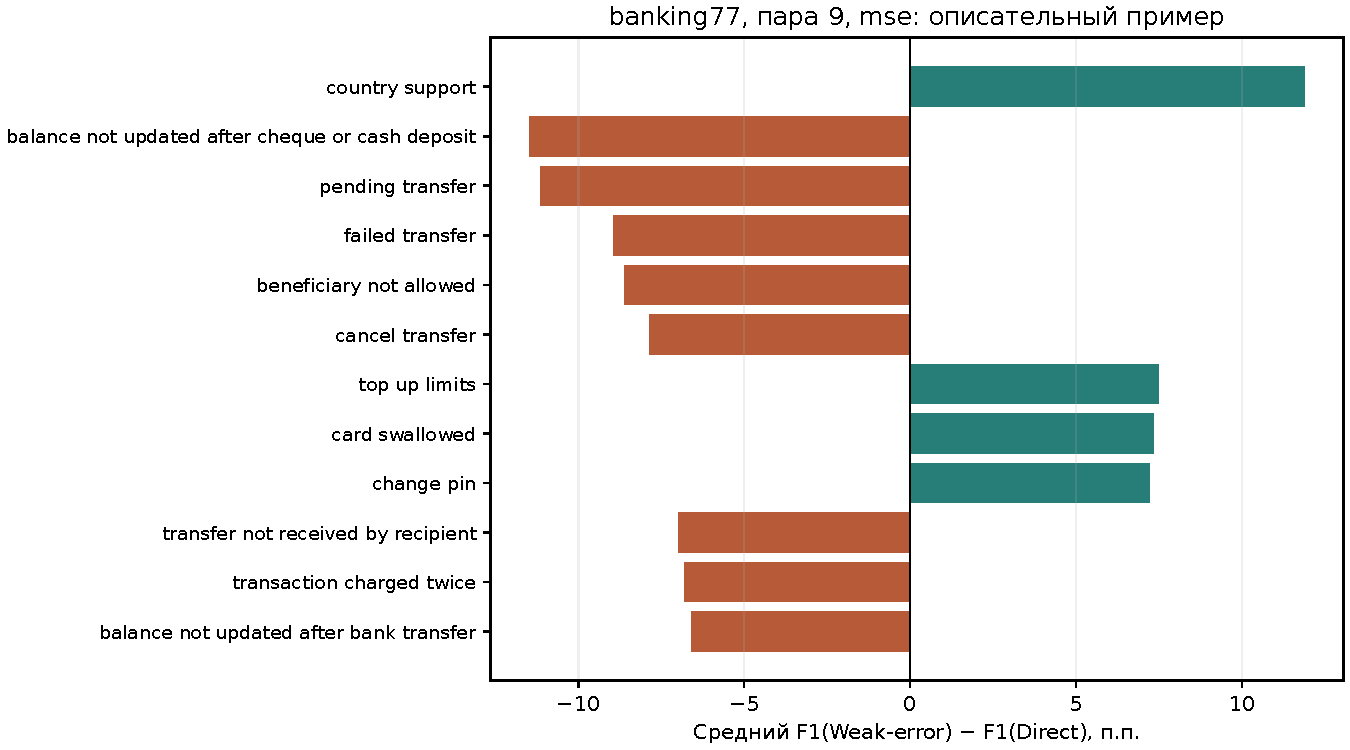
\includegraphics[width=.94\linewidth]{additions/figures/class_profile.pdf}
\caption{Описательный профиль Weak-error минус Direct,
BANKING77, TF--IDF с одной меткой на класс $\to$ tuned MiniLM.
Показаны 12 классов с наибольшим абсолютным расхождением
среднего F1; классовые p-values не вычислялись.}
\label{fig:class_extended}
\end{figure}

\section{Обсуждение: условия выбора и границы результата}
\paragraph{Что следует учитывать при выборе.}
Проверенные эффекты поддерживают выбор по сочетанию трёх характеристик:
механизма формирования парной разметки, реализованной параметризации
полезности и эксплуатационной квоты. Сравнительная деградация
gain-методов против Weak-error повторяется на втором датасете;
внутри gain-семейства найдены конкретные преимущества и взаимодействия.
Корректировка известного отбора даёт отдельный измеримый прирост,
поэтому raw-победитель и победитель среди корректно обученных
кандидатов отвечают на разные вопросы.

Практически это означает: сохранять простой обучаемый baseline,
проверять попарные взаимодействия с механизмом отбора, сравнивать
IPW и raw на одинаковых извлечениях и оценивать окончательный
выбор на отдельном dev при нужной квоте. Полученные условия
предпочтительности являются локальными ориентирами для такой процедуры,
а не правилом всегда выбирать Weak-error, Hurdle или Ternary.

\paragraph{Как интерпретировать неподтверждённые сравнения.}
Полная проверка сохраняет важные границы: в семье B natural-различия
и gain-only взаимодействия не прошли поправку; в C не установлены
прямое преимущество accuracy-настройки над MSE или надёжная смена
знака преимущества между natural и harm8. В семье M найден один
контраст методов по accuracy и macro-F1; случаев различимой macro-P/F1
при необнаруженной accuracy-разнице в той же семье нет.
Эти результаты ограничивают область утверждений, но не отменяют
конкретных эффектов таблицы~\ref{tab:main_effects}.
Незначимость не доказывает эквивалентности; разные статусы значимости
не заменяют прямой тест различия эффектов.

\paragraph{Функциональный класс и критерий настройки.}
Direct --- линейный ridge-прогноз; Hurdle --- произведение двух
logistic-голов. Поэтому найденные различия относятся к полным
реализованным способам обучения и могут включать вклад ёмкости,
потерь и регуляризации. Accuracy-настройка меняет выбранную
регуляризацию примерно в 38--48\% случаев в рассмотренных основных
срезах, но сама смена tuning-критерия не получила подтверждённого
преимущества после общей поправки. Восемь gain-only взаимодействий
относятся именно к заданному accuracy-tuned протоколу;
их наличие не является доказательством превосходства этого критерия.

\paragraph{Обобщение и статистический статус.}
BANKING77 повторно использовался после просмотра исходных результатов;
CLINC150 добавлен по отдельному плану, но его multiclass-разбор
выполнен уже после основных экспериментов. Выбранные иллюстрации
не образуют новую подтверждающую выборку. Панели внутри датасетов
зависимы, bootstrap условен на пулах, экспертах и обученных scores,
а два intent-датасета не представляют всё разнообразие задач routing.
Квота измеряет число вторых вызовов, не фактические денежные затраты
или end-to-end latency. Отбор по парным исходам предполагает,
что разметка полного пула уже приобретена.

\paragraph{Следующий содержательный контроль.}
Для отделения обучающей цели от функционального класса нужен
одинаковый Hurdle-подобный нелинейный score, обученный либо прямой MSE
на приросте, либо факторизованными потерями, с одинаковыми признаками,
регуляризацией и tuning-бюджетом. Затем критерий выбора по условной
структуре ошибок и устойчивости границы квоты следует зафиксировать
на development-данных и проверить на новой задаче. Этот контроль
ещё не выполнялся; настоящие результаты задают его мотивацию
и измеримые эффекты, которые требуется объяснить.

\section{Заключение}
Контролируемое сравнение восьми способов обучения маршрутизатора
на BANKING77 и CLINC150 установило конкретные режимы сравнительной
деградации и выигрыша. При harm-отборе без коррекции изменение
разности Direct--Weak-error равно \BankShiftEffect{} п.п.
в примере BANKING77 и \ClincShiftEffect{} п.п. в примере
CLINC150, то есть Direct теряет относительное качество.
Во втором датасете найдены также различия внутри
gain-семейства: Hurdle превосходит Direct в harm8 raw на
\HurdleSimpleEffect{} п.п., а взаимодействие метода и состава
составляет \HurdleShiftEffect{} п.п. Все восемь обнаруженных
при accuracy-настройке gain-only взаимодействий устойчивы
к численному уточнению bootstrap.

Коррекция известных вероятностей отбора повышает accuracy Direct
на \CorrectionEffect{} п.п. относительно raw в рассмотренной
CLINC-паре. Дополнительный multiclass-анализ фиксированных решений
устанавливает преимущество Ternary над Hurdle в одном natural-режиме:
\NaturalAccuracyEffect{} п.п. accuracy и \NaturalFoneEffect{} п.п.
macro-F1. Эти результаты дают положительное содержание выбору
способа обучения: важны не только средние на естественном составе,
но и чувствительность реализованного оценивателя к формированию
разметки и корректность сравнительных контролей.

Теоретическое условие смены top-$k$ связывает возможный отказ
с условными harm-вероятностями и зазорами около границы квоты.
Вместе с эмпирическими эффектами оно задаёт направление дальнейшего
исследования: сопоставить одинаковые функциональные классы
и оценить заранее заданное правило выбора на новых задачах.

